% Define block styles
\tikzstyle{blockL} = [draw, rectangle, text centered, minimum height=8.0cm, rounded corners=true]
\tikzstyle{blockL2} = [draw, rectangle, text centered, minimum height=4.0cm, rounded corners=true]
\tikzstyle{blockS} = [text centered, text width=1.0cm, minimum height=0.5cm, rounded corners=true, fill=white]
\tikzstyle{arrowtext} = [text width=4em, text centered]
\tikzstyle{arrow} = [draw, -latex]

\tikzstyle{blockT} = [text centered, text width=7.0cm, fill=white]

\definecolor{red1}{RGB}{160,0,0}
\definecolor{green1}{RGB}{0,160,0}
\definecolor{blue1}{RGB}{0,0,160}

\pgfdeclareimage[width=7.0cm]{picFlow}{./figures/robot/method_systemstructure_features_frame.jpg}
\pgfdeclareimage[width=9.0cm]{picTransform}{./figures/robot/method_systemstructure_transform_canyonfeatures.jpg}
\pgfdeclareimage[width=0.75cm]{picRottrans}{./figures/robot/method_systemstructure_rottrans.png}
\pgfdeclareimage[width=5.0cm]{picDepth}{./figures/robot/method_systemstructure_triangulation.png}
\pgfdeclareimage[width=4.0cm]{picCloud}{./figures/robot/method_systemstructure_pointcloud_small.jpg}

\usetikzlibrary{positioning}
\usetikzlibrary{fit}

  
\newsavebox\mybox
\begin{lrbox}{\mybox}
  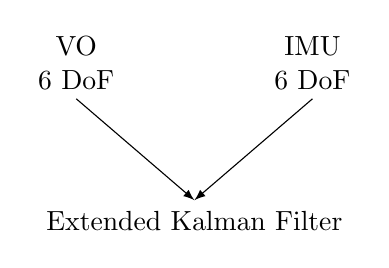
\begin{tikzpicture}[node distance=3cm, auto]
    \node [blockS] (s1) {\normalsize{VO\\6~DoF}};
    \node [blockS, right of=s1] (s2) {\normalsize{IMU\\6~DoF}};
    %\node [blockS, below of=s1, node distance=1cm] (s4) {\pgfuseimage{picRottrans}};
    \node [blockS, below of=s1, xshift=1.5cm, node distance=2.0cm, text width=4cm] (s3) {\normalsize{Extended Kalman Filter}};

    \draw [arrow] (s1.south) to (s3.north);
    \draw [arrow] (s2.south) to (s3.north);
  \end{tikzpicture}
\end{lrbox}

	      
\begin{tikzpicture}[node distance=4.5cm, auto]
  \node [] (i1) {\pgfuseimage{picFlow}};
  \node [blockT, below of=i1, node distance=4.0cm, text width=7.0cm] (t1) {a) Compute features and optical flow};

  \node [right of=i1, node distance=9.2cm] (i2) {\pgfuseimage{picTransform}};
  \node [blockT, right of=t1, node distance=9.5cm, text width=10.0cm, yshift=1.2em] (t2) {b) Transform from mirror to robot coordinate system \&\\compute 6~DoF pose (not all features shown for visualization purposes)};

  \node [below of=i1, node distance=7.5cm, xshift=-1.35cm] (i3) {\usebox\mybox};
  \node [blockT, below of=i3, node distance=2cm, text width=4.4cm] (t3) {c)~Fuse~VO~and~IMU~via~EKF};

  \node [right of=i3, node distance=6.0cm] (i4) {\pgfuseimage{picDepth}};
  \node [blockT, right of=t3, node distance=6.0cm] (t4) {d) Compute depth via triangulation};

  \node [right of=i4, node distance=6.5cm] (i5) {\pgfuseimage{picCloud}};
  \node [blockT, right of=t4, node distance=6.5cm] (t4) {e) Generate point cloud};

  \node[blockL,  below of=i1, node distance=0cm, yshift=-0.25cm, text width=7.25cm] (b1) {};
  \node[blockL,  below of=i2, node distance=0cm, yshift=-0.25cm, text width=9.25cm] (b2) {};
  \node[blockL2, below of=i3, node distance=0cm, yshift=-0.3cm, text width=4.5cm] (b3) {};
  \node[blockL2, below of=i4, node distance=0cm, yshift=-0.3cm, text width=5.25cm] (b4) {};
  \node[blockL2, below of=i5, node distance=0cm, yshift=-0.3cm, text width=5.25cm] (b5) {};

  \draw [arrow] (b1.east) to (b2.west);
  \path [arrow] (b2.south) -| ++(0.0cm,-0.75cm) -| ++(-12.05cm,0.0cm) -| ++(0.0cm,-1.1cm);
  \draw [arrow] (b3.east) to (b4.west);
  \draw [arrow] (b4.east) to (b5.west);
\end{tikzpicture}
